
\section{Breve historia}

PostgreSQL,originalmente llamada Postgres, fue creada en la UCB (Universidad de California, Berkeley) por un profesor llamado Michael Stonebraker en 1986, como un sucesor de Ingres, un motor propiedad de Computer Associates y con el objetivo de avanzar el estado del arte en bases de datos relacionales.\\

En 1996, luego de años de desarrollo en la academia, un equipo de desarrolladores fuera de Berkeley decide liberar el proyecto y hacerse cargo de sus desarrollo, trabajando varios años hasta liberar la primera versión 6.0 en 1997.\\

Desde el inicio fue un gestor de base de datos conocido por su estabilidad y con la ayuda de cientos de desarrolladores a nivel mundial, se fueron agregando nuevas funcionalidades como control de la concurrencia, nuevos tipos de datos, mayor perfomance, etc.\\


\section{¿Quienes utilizan PostgreSQL?}

En el Perú y el mundo hay gran cantidad de empresas e instituciones que han confiado uno de sus activos más valiosos, su información, a PostgreSQL, a continuación algunos ejemplos:

\subsection{Internacionales}

\begin{itemize}
\item U.S. Agency for International Development
\item U.S. Centers For Disease Control and Prevention
\item U.S. Department of Labor
\item U.S. General Services Administration
\item U.S. State Department
\item IMDB.com, The Internet Movie Database
\item Macworld
\item Sun Microsystems
\item Red Hat
\item Apple
\item Fujitsu
\item Cisco 
\item Skype
\end{itemize}

%\subsection{Nacionales}

%\begin{itemize}
%\item Americatel Perú
%\item El Comercio
%\item La Presidencia del Consejo de Ministros
%\end{itemize}

\newpage

\section{Resumen de la Arquitectura}

PostgreSQL tiene una arquitectura que incluye diversos módulos que interactuan entre si. En el nivel más alto sigue un esquema cliente-servidor mientras que en el acceso a datos utiliza un esquema por capas.

\begin{figure}[ht!]
   \centering
   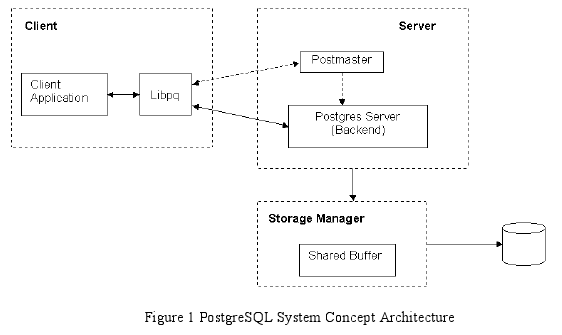
\includegraphics[scale=0.5]{imagenes/system_concept_architecture.png}
   \caption{Arquitectura de PostgreSQL}\label{graf:pg-achitecture}
\end{figure}

\begin{itemize}
\item El módulo Libpq es el encardado de gestionar las comunicaciones entre el cliente y el postmaster (servicio de PostgreSQL en el servidor).
\item El servidor esta compuesto por 2 grandes módulos, el “Postmaster” que es el responsable de aceptar las comunicaciones con el cliente, autentificar y dar acceso. El “Postgres” se encarga de administrar los querys y comandos enviados por el cliente. PostgreSQL trabaja bajo el concepto de “process per user”, eso significa un solo proceso cliente por conexión.
\item El Storage Manager (Gestor de almacenamiento) es responsable de la gestión del almacenamiento de los datos, controlar todos los trabajos del back-end incluido la administración del buffer, archivos, bloqueos y control de la consistencia de la información.
\item Cuando se guarda la data en disco, esta es utilizada para consultas. Al leer la data, se extrae del disco para pasarla a la RAM, y al escribir se transfiere de la RAM al disco. \cite{Quinones}
\end{itemize}

\subsection{Gestión de la data}

La data en todo Gestor de Bases de Datos se guarda en bloques de disco llamados “páginas” cuyo tamaño varía entre 8KB y 32KB, las cuales se guardan en diferentes posiciones físicas del disco, si se dispersan por el disco, causan menor rendimiento de la base de datos.\\	

\begin{figure}[ht!]
   \centering
   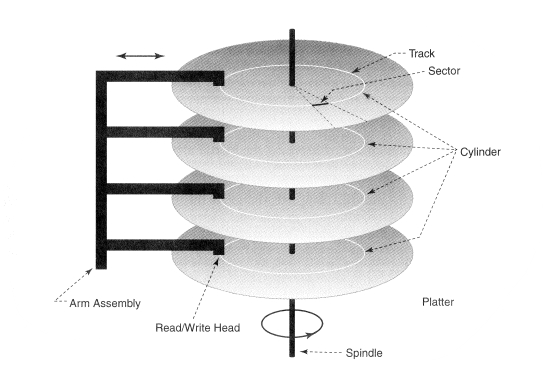
\includegraphics[scale=1]{imagenes/disk_structure.jpg}
   \caption{Estructura del disco}\label{graf:disk-achitecture}
\end{figure}

En PostgreSQL cuando se realizan operaciones de lectura y/o escritura primero se consulta al Buffer (RAM) si contiene la página, en caso no ser así, se obtiene del disco.\\

Toda operación hace que PostgreSQL agregue data. Cuando se elimina un registro o se modifica, PostgreSQL almacena una copia invisible hasta que ejecuta VACUUM y se libera de toda la data sobrante.\\

\subsubsection{Índices}

En los discos la data se almacena en bloques de datos llamados páginas, estos bloques son accedidos por entero (operación atómica). Estos bloques están estructurados como listas enlazadas, contienen una sección de data y un puntero a la localización del siguiente nodo. \\

Debido a que los registros se buscan por campos, buscar en un conjunto de campos es necesario para encontrar los registros que se buscan en una consulta, pero al buscar en un campo cuyos datos no están ordenados el tiempo de búsqueda escala junto con el tamaño de la data.\\

Un índice es un “archivo” donde esta parte de la data y estructura de una tabla con las “search key” de búsqueda. Al crear un índice en una tabla se crea otra estructura de datos que contiene el valor ordenado del campo y apunta al registro que lo contiene. Es recomendable crear índices sobre datos que se repitan lo menos posible entre si.\\

Los índices representan un gran aumento en el rendimiento de un gestor de base de datos pero consumen espacio de disco por cada índice que se cree. Debido a su capacidad de disminuir el tiempo de búsqueda en grandes tablas, solo debe ser utilizado con ese fin. \\

\begin{figure}[ht!]
   \centering
   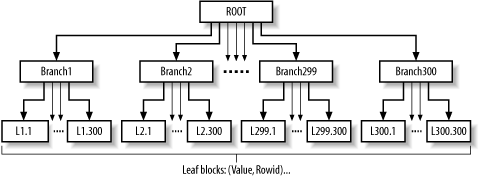
\includegraphics[scale=0.5]{imagenes/index.png}
   \caption{Índices}\label{graf:indice}
\end{figure}

\newpage


\subsection{El procesamiento de una consulta}

\begin{figure}[ht!]
   \centering
   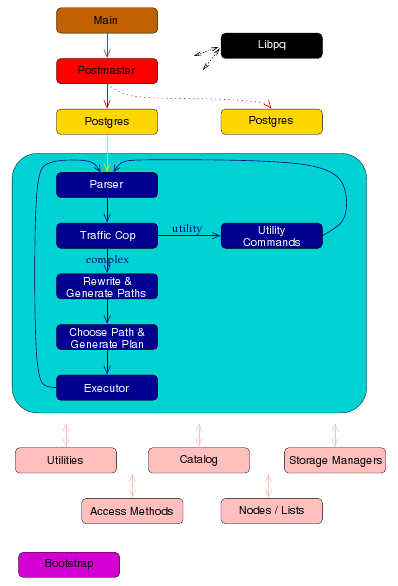
\includegraphics[scale=0.8]{imagenes/proceso_query.png}
   \caption{Procesamiento de una consulta \cite{Quinones}}\label{graf:proceso-consulta}
\end{figure}

El cliente (libpq) se comunica con el servicio del “postmaster” para pasarle una cadena de texto con la consulta. \\

El parser transforma la consulta en una serie de instrucciones que la base de datos puede interpretar, por eso es importante escribir bien las consultas.\\

A continuación se analiza que lo escrito sea sintácticamente correcto y se descompone por token la consulta para pasarla a la estructura que le corresponde (select, update, grant, etc).\\

El módulo Traffic Cop contiene al controlador principal del proceso del PostgreSQL, además se encarga de las comunicaciones entre el Parser, Optimizer, Executor y commands functions. Las consultas complejas pasan al Rewriter (select,insert, etc.), las que no, se pasan al Utility Commands, en general consulta simples (alter, create, vacuum, etc).\\

El módulo “planner” es el encargado de generar el “plan de ejecución”, esto es estimar la mejor vía para resolver el query, maneja mediante formulas matemáticas avanzadas la forma de búsqueda de datos y la forma de resolver las relaciones entre tablas. Luego que el planner calcula la forma más eficiente de ejecutar la consulta se la pasa al “Executor” que la lleva a cabo. \cite{Quinones}


\section{Multi-Version Concurrency Control (MVCC)}

Una decisión de diseño importante que se debe tomar en toda BD es como gestionar la interacción de múltiples clientes con la misma data. PostgreSQL utiliza un enfoque llamado Multiversion Concurrency Control (control multiversión de la concurrencia) el cuál es también utilizado en otras Bds como Oracle.\\

Mediante el control de concurrencia el gestor permite que muchos usuarios puedan acceder a la misma data al mismo tiempo. Cada proceso de usuario ejecuta transacciones las que a su vez pueden contener una o más operaciones.\\

Las transacciones deben cumplir el criterio ACID:\\

\begin{itemize}
\item \textbf{A tomicity}: todas las acciones en la transacción se cumplen o no se cumple ninguna.
\item \textbf{C onsistency}: la transacción solo termina si la data es consistente.
\item \textbf{I solation}: la transacción es independiente de otras transacciones.
\item \textbf{D urability}: cuando la transacción termina el resultado de la misma permanece.
\end{itemize}

Bajo el MVCC, la implementación de concurrencia de PostgreSQL, las transacciones ven una imagen de la data al momento de
empezar (para eso la data se versiona con un timestamp), esto protege la transacción de inconsistencia de data cuando llegan varias operaciones de Lectura/escritura sobre el mismo registro.\\

La data no se modifica o elimina, solo se agregan nuevos registros y los antiguos pasan a ser invisibles. La nueva data no es visible para otras transacciones hasta que no termina la actual transacción y es enviada (committed) a la base de datos.


\section{Write-Ahead Logging}

Es el método estándar en los gestores de bases de datos para asegurar la integridad de la data. El concepto central de WAL es que los cambios a los archivos de data (donde las tablas y los índices residen) solo deben ser escritos después que los cambios han sido registrados, esto es, después de que los registros de logs describiendo los cambios se hayan guardado de forma permanente. Esto sirve para que en caso de un desastre, se pueda recuperar la Bd utilizando el log del servidor.\\

El parámetro \textit{wal\_level} de \textit{postgresql.conf} determina cuanta información es registrada en el WAL. Las alternativas son tres: minimal (opción por defecto), archive y hot\_standby.\\

En el nivel minimal, no se registran algunas operaciones como CREATE TABLE AS o CREATE INDEX pero este nivel no guarda suficiente información como para reconstruir la data de la BD desde el WAL.\\

Para poder llevar a cabo replicación se necesita utilizar los niveles \textit{archive} o \textit{hot\_standby}. La diferencia entre ambos es que hot\_standby no solo registra todos los cambios en la data sino además las transacciones así sea de solo lectura

\section{Objetos más utilizados en PostgreSQL} 
\begin{itemize}
\item El servidor PostgreSQL también conocido como servidor o demonio, se puede tener más  de uno en un servidor siempre y cuando utilicen diferentes puertos o ips y almacenen su data en ubicaciones diferentes.
\item Base de datos, cada servidor puede tener varias bases de datos.
\item Tablas, son la principal herramienta de toda base de datos.
\item Esquemas, son parte del estándar ANSI-SQL, y son los contenedores lógicos de tablas y otros objetos. Cada base de datos puede tener diferentes esquemas.
\item Tablespace, es la localización física donde la data es almacenada. Postgresql permite que se gestionen de forma independiente, lo que significa que se pueden mover las bases de datos a otras particiones o discos con pocos comandos.
\item Vistas, se utilizan para abstraer las consultas y en PostgreSQL además pueden ser actualizadas.
\item Funciones, en Postgresql pueden retornar un solo valor o un set de registros. 
\item Operador, son funciones simbólicas que tienen el respaldo de una función, en PostgreSQL se pueden definir por el usuario.
\item Cast, permite convertir de un tipo a otro y es soportado por funciones que realmente hacen la conversión. En PostgreSQL los usuarios pueden crear sus propias funciones de conversión.
\item Sequence, controlan los números autoincrementales en las definiciones de las tablas. Se crean automáticamente cuando se define una columna serial.
\item Triggers, son los disparadores de acciones al detectar cambios en la data.
\item Data externa, en postgresql se puede hacer consultas fuentes externa de data ya sea que esa fuente sea otra BD relacional, un archivo plano, una Bd NoSql, un web service, etc.
\item Extensiones, agrupan funciones, tipos, casts, indices en una sola unidad para mayor mantenibilidad. Es sobre todo usar para instalar módulos adicionales.
\end{itemize}

\section{Nuevas funcionalidades en PostgreSQL 9.2}

Algunas de las nuevas funcionalidades de Postgresql 9.2 son: \cite{Obe2012}

\begin{itemize}
\item Acelerar la consulta de columnas pertenecientes a un index.
\item Mejoras en el ordenamiento que optimizan operaciones de ordenamiento en memoria hasta un 20\%.
\item Mejoras en el planeamiento de consultas.
\item Replicación en cascada ahora soporta streaming de un esclavo a otro esclavo.
\item ALTER TABLE IF EXISTS sintaxis para hacer cambios en tablas.
\item Más opciones para ALTER TABLE.
\item Más opciones para crear y restaurar backups.
\item La posibilidad de crear funciones en javascript mediante plv8js.
\item El tipo JSON como tipo nativo de Postgresql.
\item Las funciones SQL pueden referirse a los argumentos por nombre y no por número.

\end{itemize}

\section{Limitaciones}

PostgreSQL por su naturaleza de BD para servidores, no es aplicable para ser embebida como SQLite o Firebird. Además, en muchos hostings por uno u otro motivo no está presente PostgreSQL, aunque ese es un problema que se está solucionando con el tiempo.

\section{Instalación}

Para instalar en Ubuntu la versión 9.2 de PostgreSQL llevamos a cabo los siguientes pasos:

\begin{itemize}
\item Instalar las librerías requeridas
\begin{itemize}
\item \textbf{sudo apt-get install libpq-dev}
\end{itemize}
\item Agregar el repositorio donde está ubicado PostgreSQL 9.2 (no está aún en los repositorios oficiales).
\begin{itemize}
\item \textbf{sudo add-apt-repository ppa:pitti/postgresql}
\end{itemize}

\item Actualizar la lista de paquetes disponibles:
\begin{itemize}
\item \textbf{sudo apt-get update}
\end{itemize}

\item Instalar el servidor

\begin{itemize}
\item \textbf{sudo apt-get install postgresql-9.2}
\end{itemize}

\end{itemize}

Poner a punto el servidor:

\begin{itemize}
\item Ingresar en el template1 de Postgresql para cambiar la contraseña del usuario por defecto.
\begin{itemize}
\item \textbf{sudo su postgres -c psql template1}
\end{itemize}

\item Cambiar la contraseña del usuario postgres.
\begin{itemize}
\item \textit{postgres=\# ALTER USER postgres WITH PASSWORD 'qwerty';}
\end{itemize}

\item Salimos del cliente psql.
\begin{itemize}
\item $\backslash$q
\end{itemize}

\item Eliminamos la contraseña del usuario postgres en el sistema
\begin{itemize}
\item \textbf{sudo passwd -d postgres}
\end{itemize}

\item Se utiliza su para cambiar el password del usuario postgres
\begin{itemize}
\item \textbf{sudo su postgres -c passwd}
\end{itemize}

\item Se crea el usuario “pedro” con el usuario del servidor postgres
\begin{itemize}
\item \textbf{sudo -u postgres createuser -D -A -P pedro}
\end{itemize}

\item Crear la DB 
\begin{itemize}
\item \textbf{sudo -u postgres createdb -O pedro Bd\_prueba}
\end{itemize}

\end{itemize}

Para instalar Pgadmin:

\begin{itemize}
\item \textbf{sudo apt-add-repository ppa:voronov84/andreyv}
\item \textbf{sudo apt-get update}
\item \textbf{sudo apt-get install pgadmin3}
\end{itemize}

\begin{figure}[ht!]
   \centering
   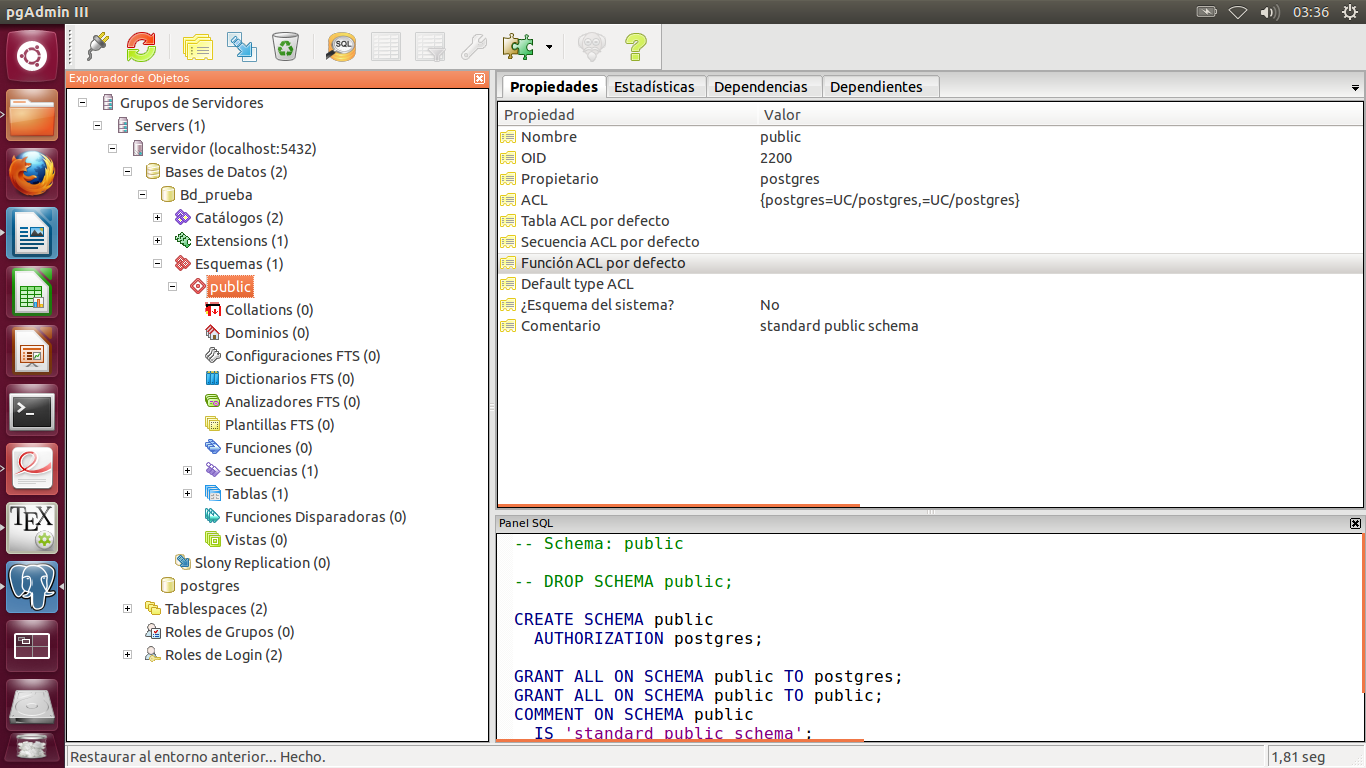
\includegraphics[scale=0.35]{imagenes/pgadmin3.png}
   \caption{Pantalla principal de Pgadmin3}\label{graf:pgadmin3}
\end{figure}

\subsubsection{Auto Explain}

Otra opción muy utilizada después de la versión 8.4 de PostgreSQL es el módulo auto\_explain que permite analizar la duración de una consultada viendo su plan EXPLAIN asociado.\\

Para habilitarlo se debe agregar en postgresql.conf los siguientes parámetros y reiniciar el servidor:\\

\emph{shared\_preload\_libraries = 'auto\_explain'\\
custom\_variable\_classes = 'auto\_explain' \\
auto\_explain.log\_min\_duration = '1s'\\}

Esta configuración va a ejecutar auto\_explain en toda consulta que dure más de un segundo registrándola con un plan EXPLAIN completo.



\newpage

Ejercicios:

\begin{enumerate}
\item Instalar el servidor Postgresql.
\item Crear una base de datos llamada Base\_curso.
\item Crear un usuario llamado “usuario\_curso”.
\item Crear la tabla Persona de propiedad del usuario “usuario\_curso” con los siguientes campos:
\item nombre, apellidop, apellidom.
\item Insertar el nombre y apellidos de tres alumnos en la tabla.
\end{enumerate}



